\begin{center}
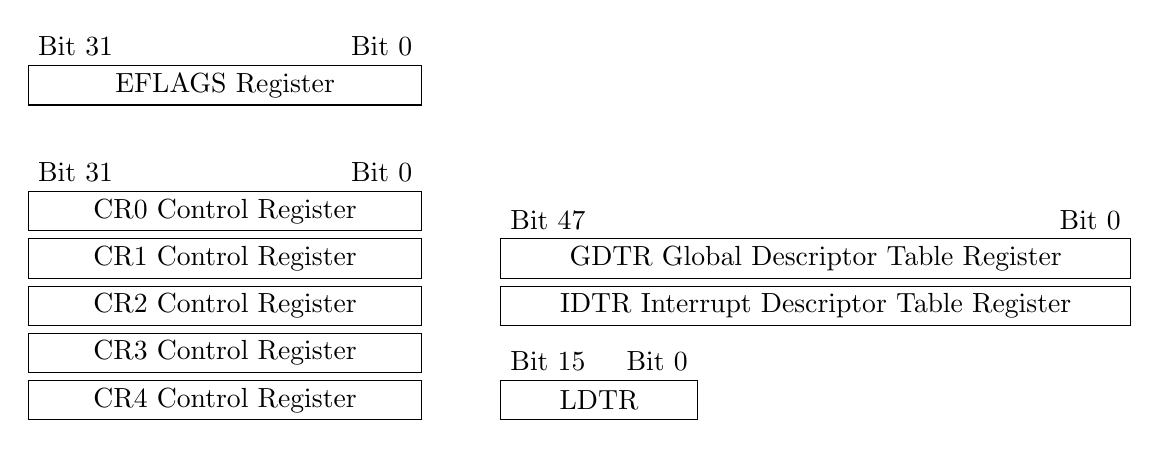
\begin{tikzpicture}
\draw (0,0) rectangle (5,0.5) node [pos=0.5] {CR4 Control Register};
\draw (0,0.6) rectangle (5,1.1) node [pos=0.5] {CR3 Control Register};
\draw (0,1.2) rectangle (5,1.7) node [pos=0.5] {CR2 Control Register};
\draw (0,1.8) rectangle (5,2.3) node [pos=0.5] {CR1 Control Register};
\draw (0,2.4) rectangle (5,2.9) node [pos=0.5] {CR0 Control Register};
\node at (0,2.9) [above right] {Bit 31};
\node at (5,2.9) [above left] {Bit 0};

\draw (0,4) rectangle (5,4.5) node [pos=0.5] {EFLAGS Register};
\node at (0,4.5) [above right] {Bit 31};
\node at (5,4.5) [above left] {Bit 0};

\draw (6,0) rectangle (8.5,0.5) node [pos=0.5] {LDTR};
\node at (6,0.5) [above right] {Bit 15};
\node at (8.5,0.5) [above left] {Bit 0};

\draw (6,1.2) rectangle (14,1.7) node [pos=0.5] {IDTR Interrupt Descriptor Table Register};
\draw (6,1.8) rectangle (14,2.3) node [pos=0.5] {GDTR Global Descriptor Table Register};
\node at (6,2.3) [above right] {Bit 47};
\node at (14,2.3) [above left] {Bit 0};
\end{tikzpicture}
\end{center}